$\alpha = \beta = 1$, $t_f\to \infty $ and $H = 0$



Riccati equation:
\begin{equation}\label{riccati_equation}
	\dot{K} + KA +A^TK - KBR^{-1}B^TK + Q = 0
\end{equation}
\begin{equation}\label{uQ3_a}
	u(t)	= -R^{-1}B^TK(t)x(t);
\end{equation}
\begin{equation}\label{xQ3_a}
	\dot x(t) = Ax(t) + Bu(t)
\end{equation}
Because of $t \to \infty$, $\dot K = 0$ so Differential riccati equation change to Algebraic riccati equation.  
\begin{equation}\label{Al_riccati_equation}
	KA +A^TK - KBR^{-1}B^TK + Q = 0
\end{equation}
\begin{align*}
 \begin{bmatrix}
		K_{11} & K_{12} \\
		K_{21} & K_{22}
	\end{bmatrix} 
	\begin{bmatrix}
		0 & 1 \\
		-1 & -0.1
	\end{bmatrix} &+
	\begin{bmatrix}
		0 & -1 \\
		1 & -0.1
	\end{bmatrix} 
	\begin{bmatrix}
		K_{11} & K_{12} \\
		K_{21} & K_{22}
	\end{bmatrix} + \\
 \begin{bmatrix}
	K_{11} & K_{12} \\
	K_{21} & K_{22}
\end{bmatrix}  \begin{bmatrix}
0 \\
1
\end{bmatrix}
 \begin{bmatrix}
	1
\end{bmatrix}
 \begin{bmatrix}
 0 & 1
\end{bmatrix}   
 \begin{bmatrix}
	K_{11} & K_{12} \\
	K_{21} & K_{22}
\end{bmatrix} &+  \begin{bmatrix}
1 & 0 \\
0 & 1
\end{bmatrix}  =  \begin{bmatrix}
0 & 0 \\
0 & 0
\end{bmatrix} 
\end{align*}
$$
 \begin{bmatrix}\label{alrecattiequation}
	1 - K_{21} - K_{12}K_{21} - K_{12} &  K_{11} - K_{12}/10 - K_{22} - K_{12}K_{22} \\
	K_{11} - K_{21}/10 - K_{22} - K_{21}K_{22} & K_{22}^2 - K_{22}/5 + K_{12} + K_{21} + 1
\end{bmatrix} 
= \begin{bmatrix}
	0 & 0\\0 &0
\end{bmatrix}
$$
We know that $K_{12} = K_{21}$
Equation \ref{alrecattiequation} solved in MATLAB(Q3\_a.m).
There is two answer in real numbers.
$$K_1 = \begin{bmatrix} 
	-2.0175&  0.4142\\
	0.4142& -1.4556
\end{bmatrix}, \quad K_2 = \begin{bmatrix} 
1.8175&  0.4142\\
0.4142& 1.2558
\end{bmatrix}$$
Now we use equation \ref{uQ3_a} and \ref{xQ3_a} in MATLAB ode45(Q3\_aODE.m) to simulate system and find out which K is appropriate for system.
\begin{figure}[H]
	\caption{System simulation with $K_1$ matrix}
	\centering
	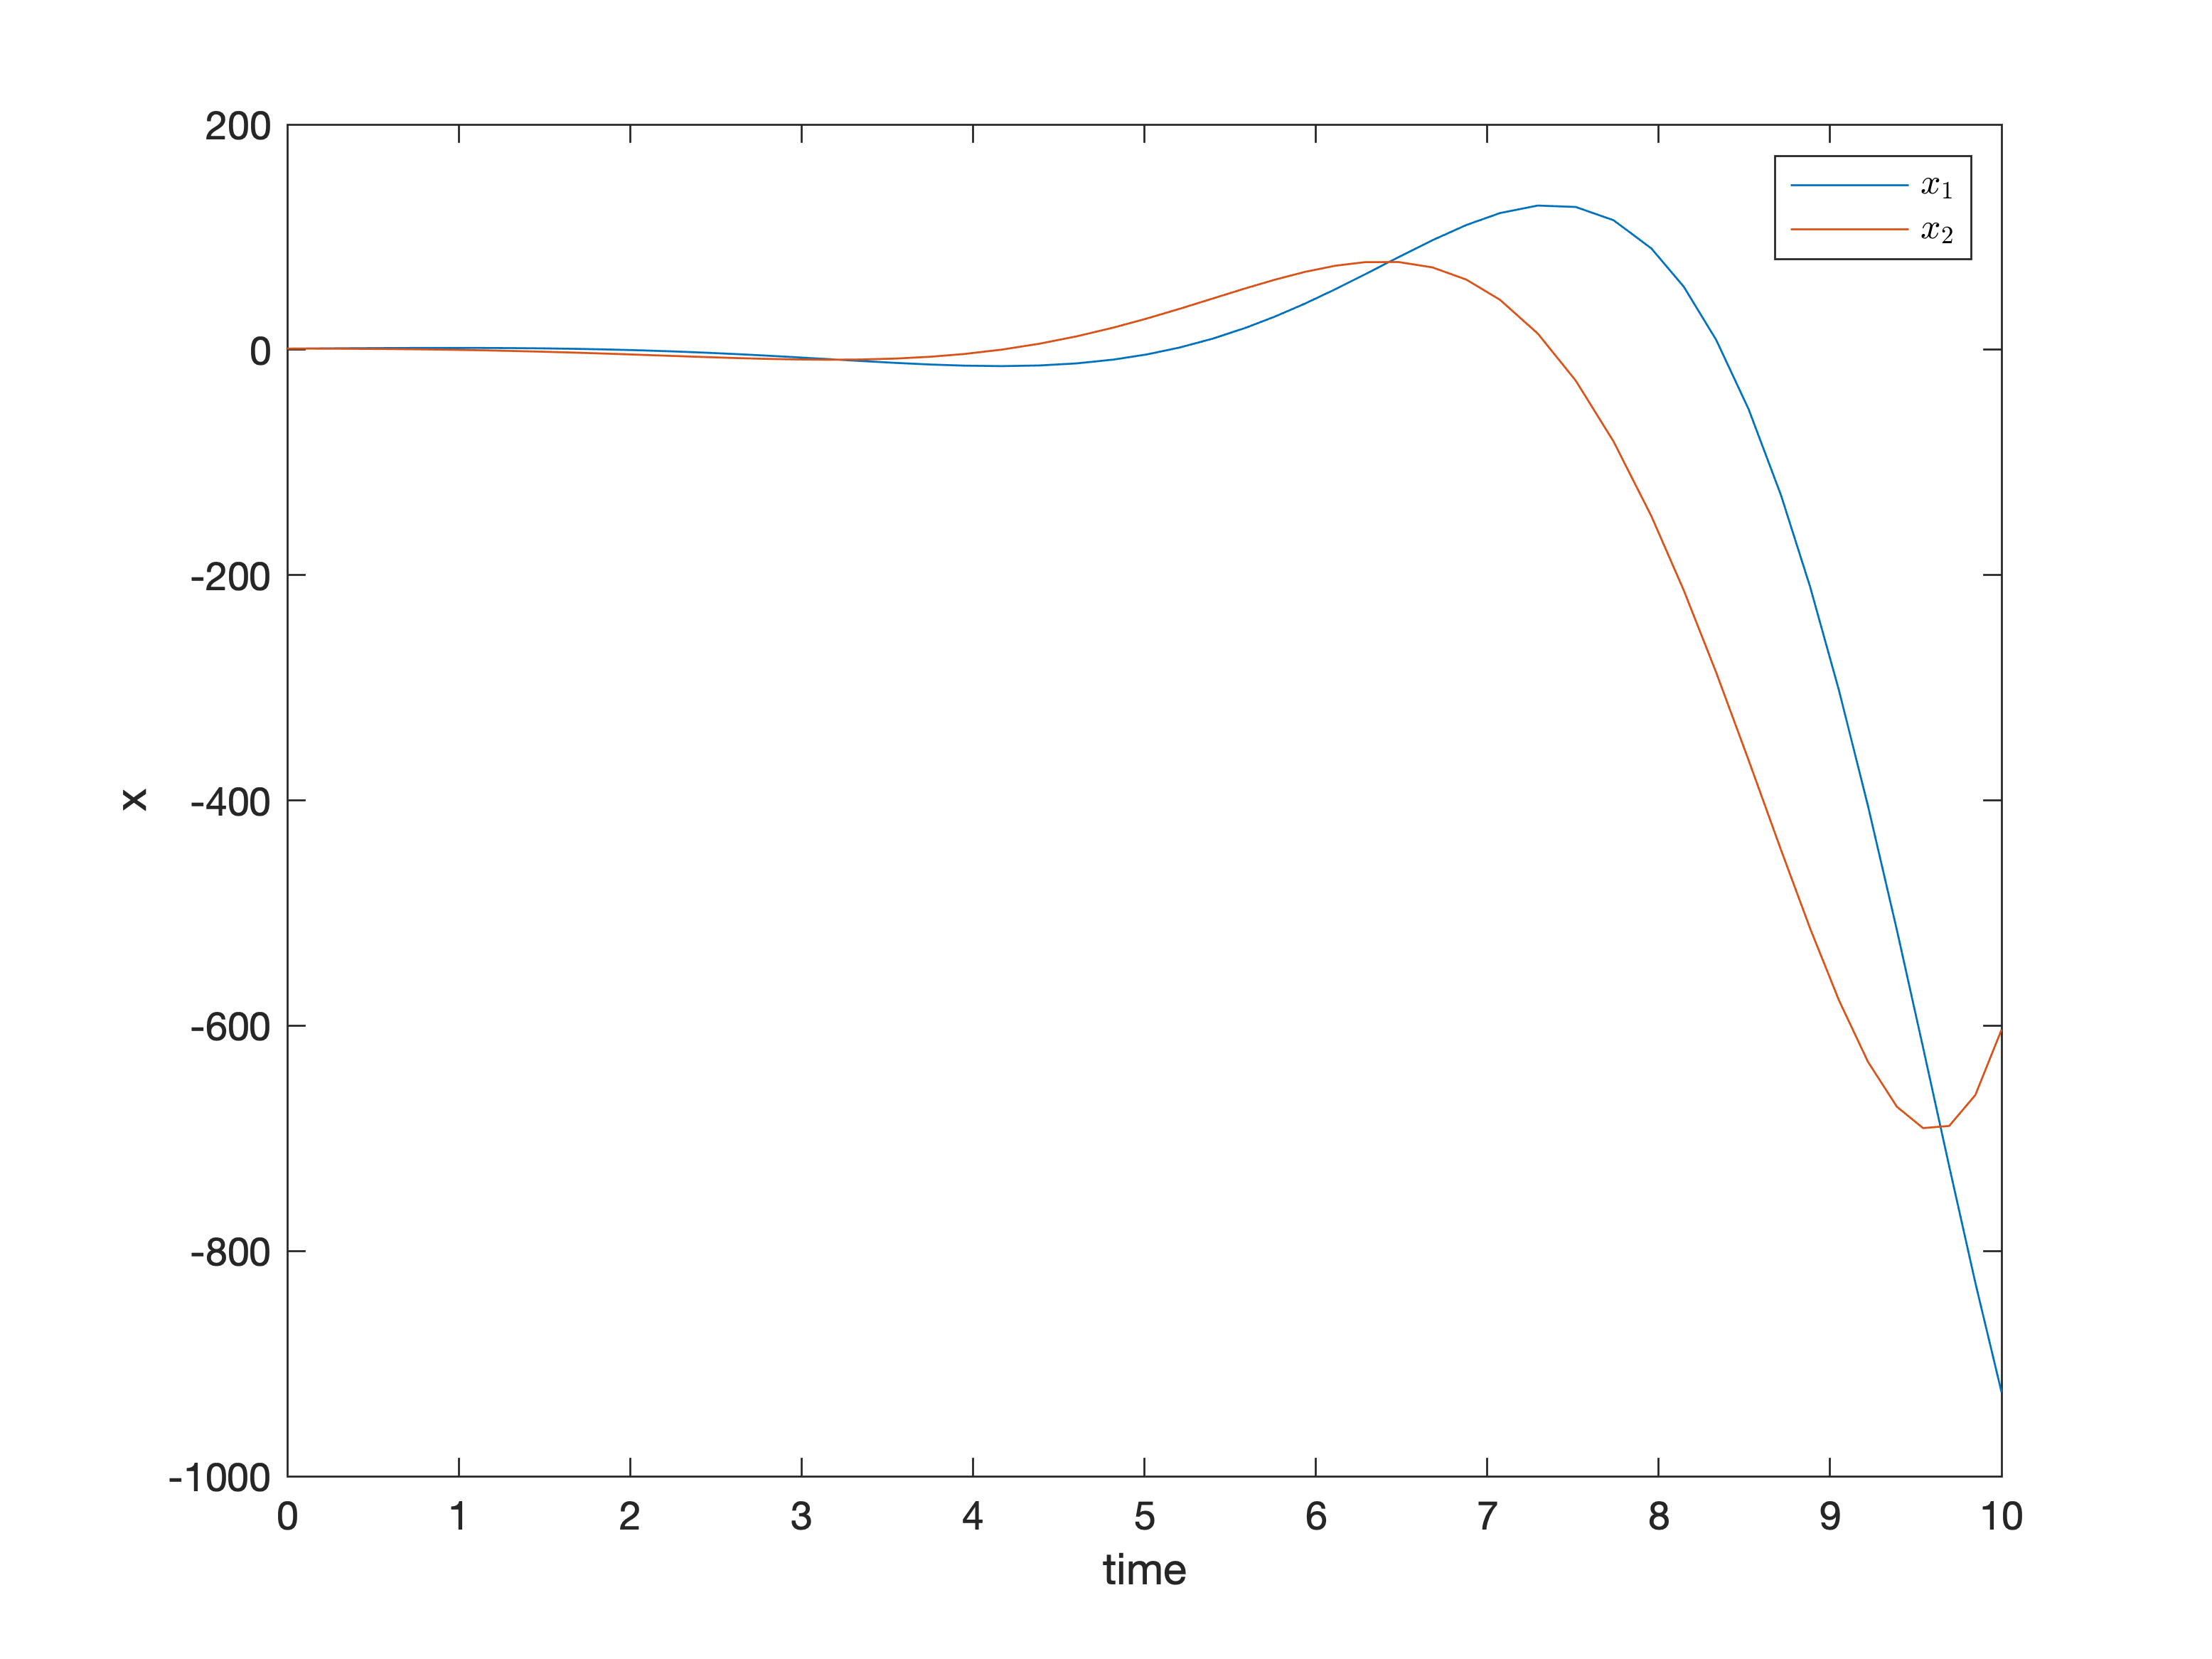
\includegraphics[width=12cm]{../Code/Q3/figures/K1ODE.png}
\end{figure}
\begin{figure}[H]
	\caption{System simulation with $K_2$ matrix}
	\centering
	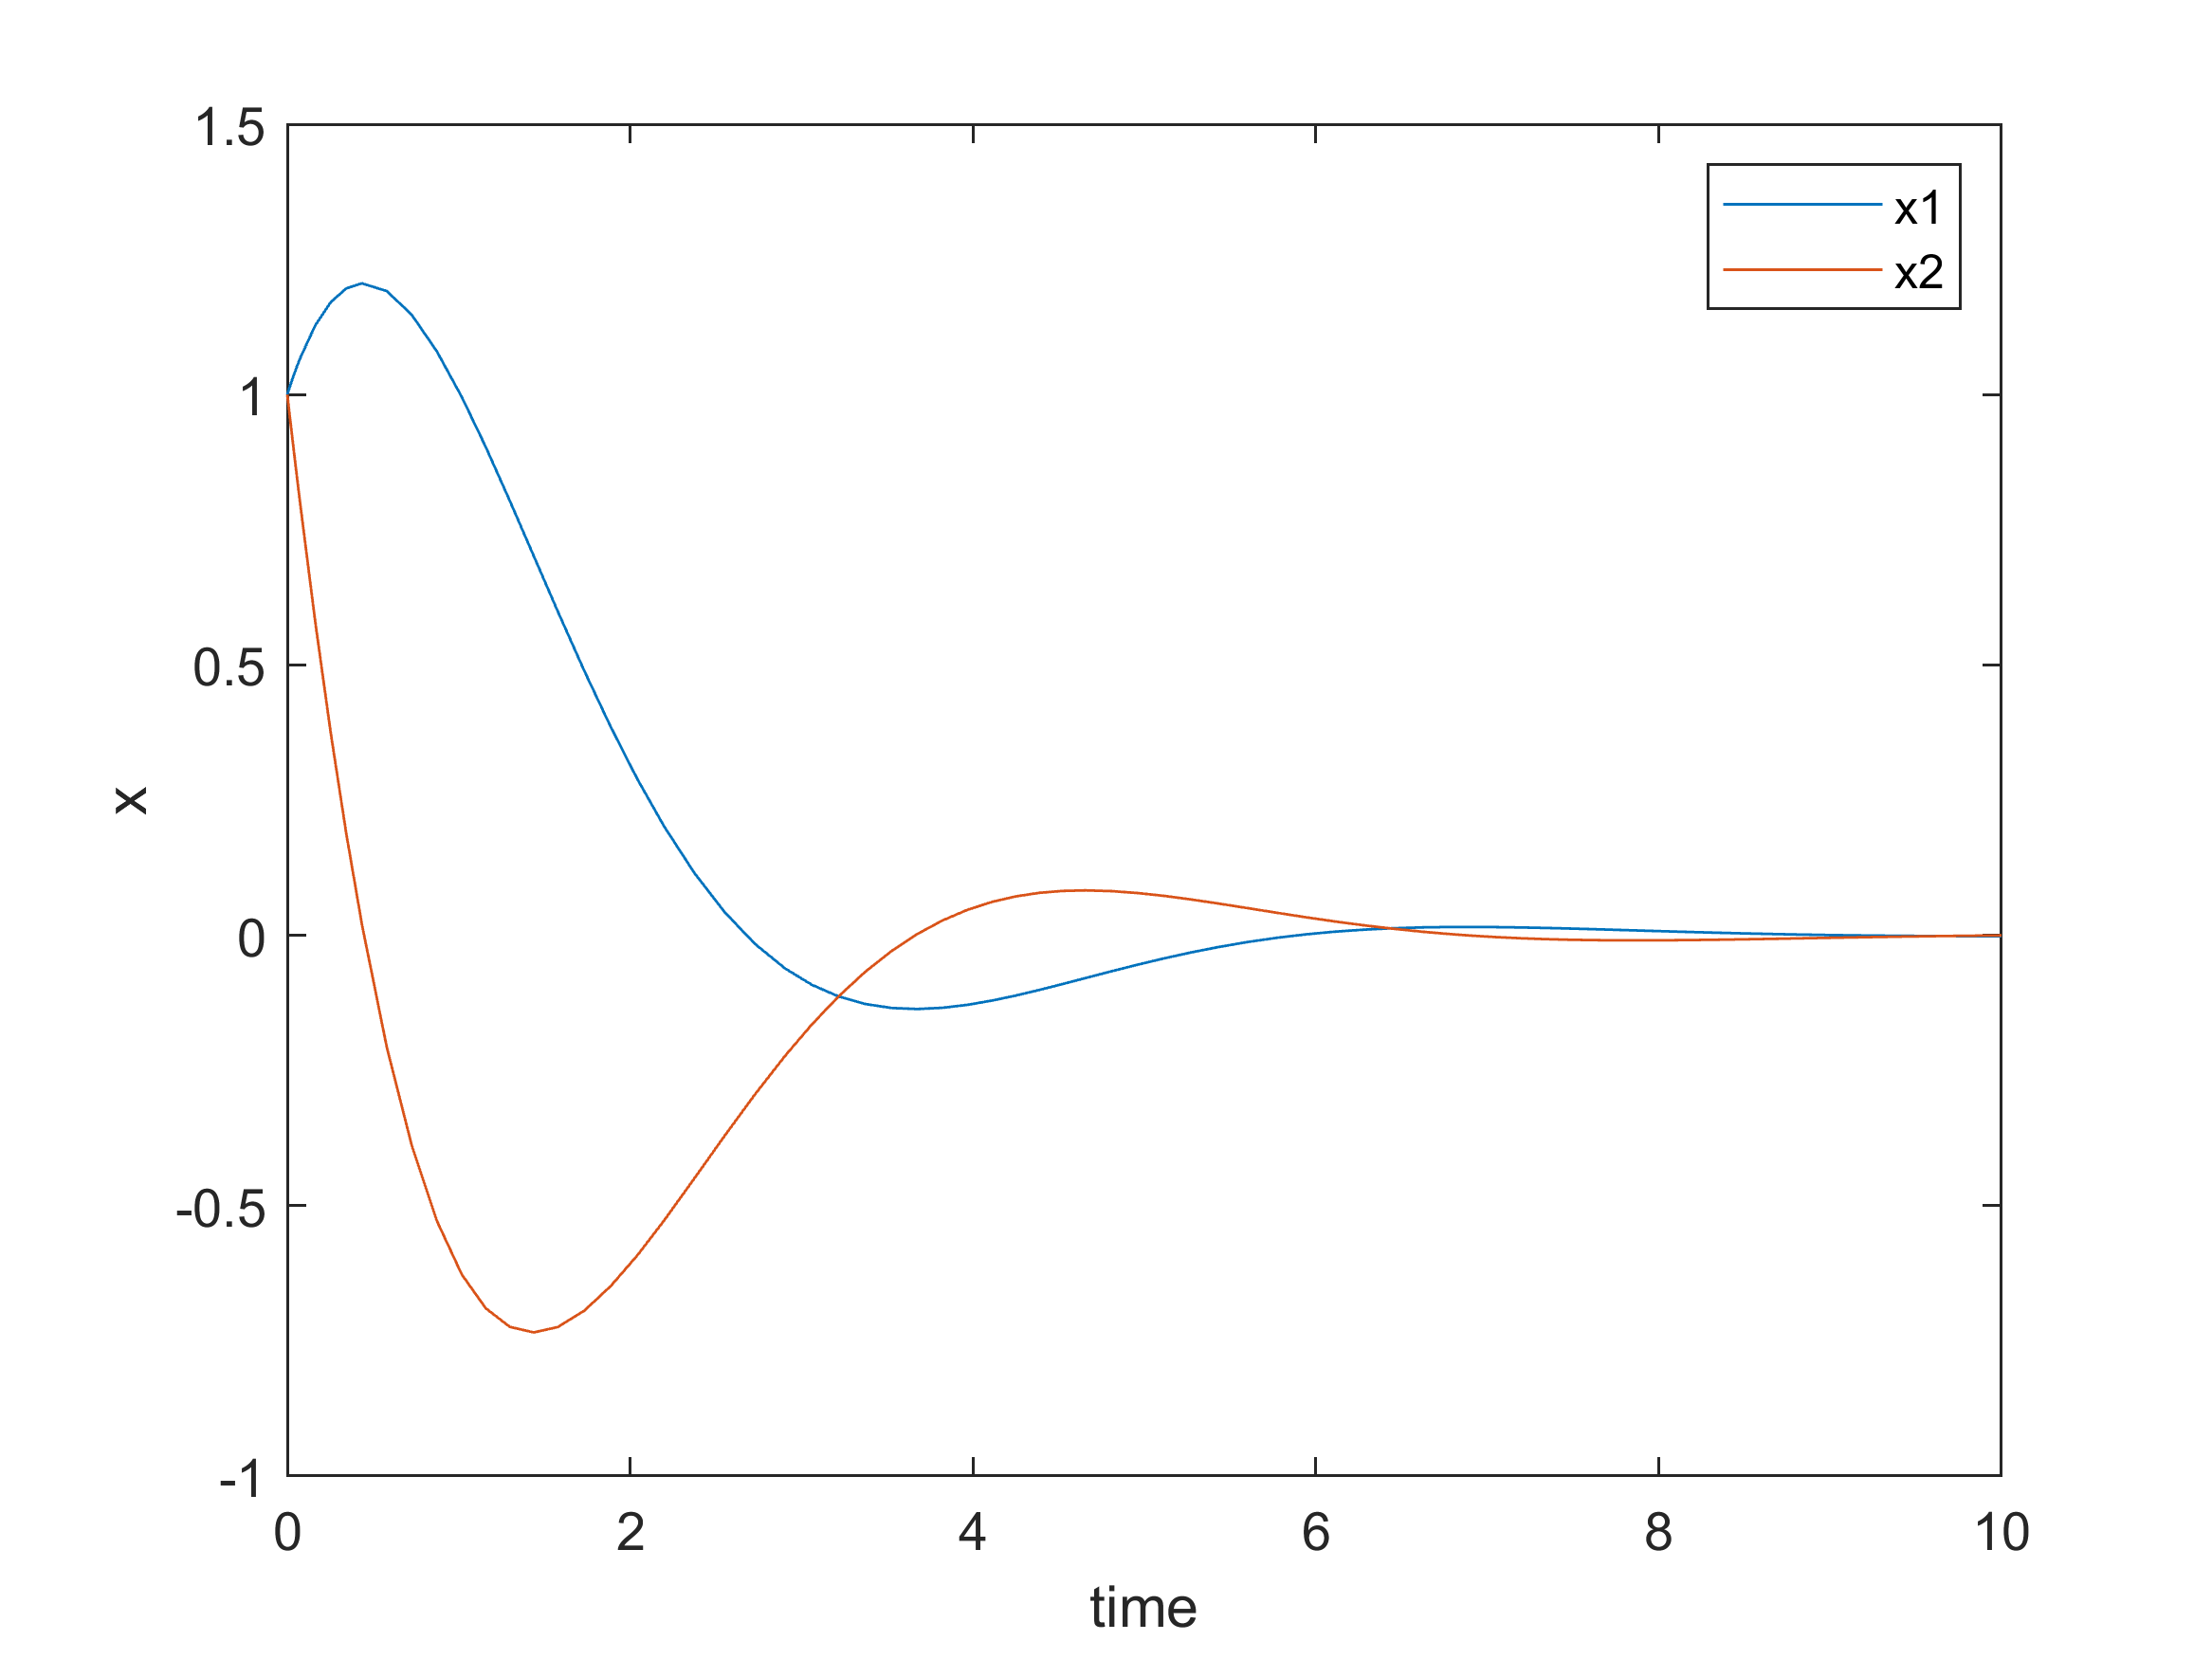
\includegraphics[width=12cm]{../Code/Q3/figures/K2ODE.png}
\end{figure}